%%%%%%%%%%%%%%%%%%%%%%%%%%%%%%%%%%%%%%%%%%%%%%%%
% chapter1.tex                                 %
% Contains formatting and content of chapter 1 %
%%%%%%%%%%%%%%%%%%%%%%%%%%%%%%%%%%%%%%%%%%%%%%%%
\chapter{Introduction and Historical Review}
\newpage

\section{Introduction}
Blah blah blah. Here is an example of how to include and cite a figure: see Figure~\ref{fig:example_figure}
\begin{figure}[H]
\center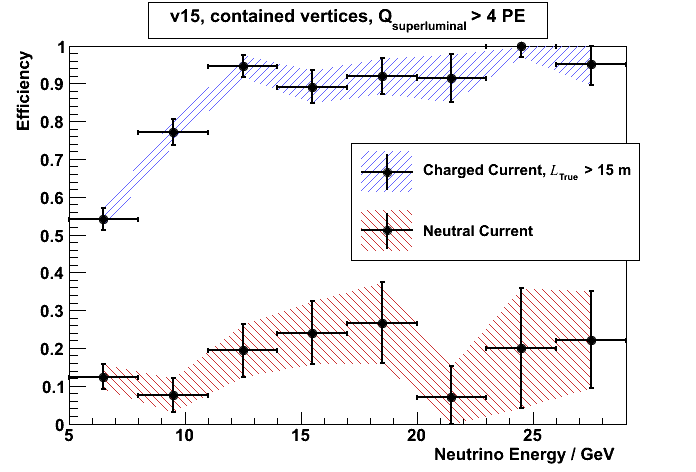
\includegraphics[width=0.4\textwidth]{figures/ExampleFigure.png}
\caption[Caption to go in list of figures]{Caption to go underneath figure}
\label{fig:example_figure}
\end{figure}

\section{Literature Review}
Blah blah blah Here's an example of a table: see Table~\ref{tab:best_values}.

\begin{table}[H]
\centering\onehalfspacing
\vline
\begin{tabular}{c c c}
\hline
\textbf{Parameter} & \vline & \textbf{Current Best Value}\\
\hline
$\Delta m^2_{21}$ & \vline & $7.50^{+0.19}_{-0.20} \times 10^{-3}\;\mathrm{eV}^2$\\
$|\Delta m^2_{32}|$ & \vline & $2.32^{+0.12}_{-0.08} \times 10^{-5}\;\mathrm{eV}^2$\\
$\sin^2{(\theta_{12})}$ & \vline & $0.857^{+0.023}_{-0.025}$\\
$\sin^2{(2\theta_{23})}$ & \vline & $>0.95$\\
$\sin^2{(\theta_{13})}$ & \vline &  $0.098\pm 0.013$\\
\hline\end{tabular}\vline
\captionsetup{width=0.86\textwidth}
\caption[Names of table for list of tables]{Name of table for caption above table}
\label{tab:best_values}
\end{table}

Here's an example of an equation and some math:
\begin{equation}
  U = \begin{pmatrix} c_{12}c_{13} & s_{12}c_{13} & s_{13}e^{i\delta}\\
    -s_{12}c_{23} - c_{12}s_{23}s_{13}e^{i\delta} & c_{12}c_{23} - s_{12}s_{23}s_{13}e^{i\delta} & s_{23}c_{13}\\
    s_{12}s_{23} - c_{12}c_{23}s_{13}e^{i\delta} & -c_{12}s_{12} - s_{12}c_{23}s_{13}e^{i\delta} & c_{23}c_{13}
  \end{pmatrix},
\end{equation}
with $c_{ij} = \cos{\theta_{ij}}$ and $s_{ij} = \sin{\theta_{ij}}$.

Here's an example citation: \citep{PDG}.

\section{Thesis Outline}

Impulsive thrust approximations are often used to simply the analysis of the optimal maneuver between circular orbits.
 In actuality, spacecraft exhibit finite thrust arcs to perform these orbital transfers. This thesis analyzes these minimum burn time, and thus fuel consumption,
 thrust arcs required for these optimal orbital transfers. Requiring two separate numerical integrations, this is computationally extensive. This thesis
 then seeks to develop methods to drastically reduce the time required for these computations through means of a C++ implementation utilizing Boost libraries and
 parallelization through OpenMP. Chapter 2 will detail the finite thrust transfer problem solved within this analysis, while Chapter 3 details the implementation details which were used.
 Chapter 4 then details the results of these implementations, including speedup comparisons and methods to greater improve the probability of the algorithm approaching an optimal solution.